% 08_rate_limiting.tex
\chapter{Rate Limiting}

Il rate limiting è una tecnica fondamentale per proteggere le API da abusi, attacchi DoS, e garantire un uso equo delle risorse. In questo capitolo esploreremo algoritmi, implementazioni e best practices.

\section{Introduzione}

\subsection{Cos'è il Rate Limiting}

Il rate limiting limita il numero di richieste che un client può effettuare in un determinato periodo di tempo.

\begin{tcolorbox}[title=Obiettivi del Rate Limiting]
\begin{itemize}
\item \textbf{Protezione da abusi}: Prevenire spam e scraping massivo
\item \textbf{Disponibilità}: Garantire che l'API rimanga disponibile per tutti
\item \textbf{Controllo costi}: Limitare l'uso di risorse computazionali
\item \textbf{Fairness}: Distribuire equamente le risorse tra gli utenti
\item \textbf{Sicurezza}: Mitigare attacchi brute-force e DoS
\end{itemize}
\end{tcolorbox}

\subsection{Livelli di Rate Limiting}

\begin{enumerate}
\item \textbf{Per IP Address}: Limita richieste da un singolo IP
\item \textbf{Per User/API Key}: Limita per utente autenticato
\item \textbf{Per Endpoint}: Limiti diversi per endpoint diversi
\item \textbf{Globale}: Limite totale di richieste all'API
\item \textbf{Per Piano}: Limiti differenziati (free, pro, enterprise)
\end{enumerate}

\section{Algoritmi di Rate Limiting}

\subsection{Fixed Window Counter}

L'algoritmo più semplice: conta le richieste in finestre temporali fisse.

\begin{center}
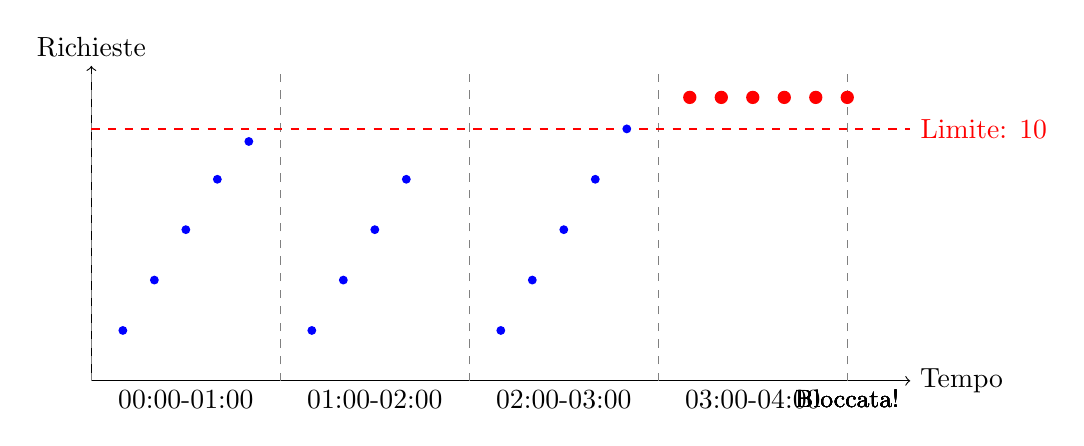
\begin{tikzpicture}[scale=0.8]
  \draw[->] (0,0) -- (13,0) node[right] {Tempo};
  \draw[->] (0,0) -- (0,5) node[above] {Richieste};

  % Finestre
  \foreach \x in {0,3,6,9,12} {
    \draw[dashed, gray] (\x,0) -- (\x,5);
  }

  % Limite
  \draw[red, thick, dashed] (0,4) -- (13,4) node[right] {Limite: 10};

  % Richieste
  \foreach \x/\y in {0.5/2, 1/4, 1.5/6, 2/8, 2.5/9.5} {
    \fill[blue] (\x, \y*0.4) circle (2pt);
  }
  \foreach \x/\y in {3.5/2, 4/4, 4.5/6, 5/8} {
    \fill[blue] (\x, \y*0.4) circle (2pt);
  }
  \foreach \x/\y in {6.5/2, 7/4, 7.5/6, 8/8, 8.5/10} {
    \fill[blue] (\x, \y*0.4) circle (2pt);
  }
  \foreach \x/\y in {9.5/2, 10/4, 10.5/6, 11/8, 11.5/10, 12/12} {
    \fill[red] (\x, 4.5) circle (3pt);
    \node[below] at (12, 0) {\small Bloccata!};
  }

  % Etichette finestre
  \node[below] at (1.5, 0) {00:00-01:00};
  \node[below] at (4.5, 0) {01:00-02:00};
  \node[below] at (7.5, 0) {02:00-03:00};
  \node[below] at (10.5, 0) {03:00-04:00};
\end{tikzpicture}
\end{center}

\subsubsection{Implementazione}

\begin{lstlisting}[language=Python, caption=Fixed Window in Python/Redis]
import time
import redis

class FixedWindowRateLimiter:
    def __init__(self, redis_client, window_seconds=60, max_requests=10):
        self.redis = redis_client
        self.window = window_seconds
        self.max_requests = max_requests

    def is_allowed(self, user_id):
        """Verifica se la richiesta e' consentita"""

        # Calcola inizio della finestra corrente
        current_window = int(time.time() / self.window)
        key = f"rate_limit:{user_id}:{current_window}"

        # Incrementa contatore
        current_count = self.redis.incr(key)

        # Imposta scadenza se e' la prima richiesta della finestra
        if current_count == 1:
            self.redis.expire(key, self.window)

        # Verifica limite
        return current_count <= self.max_requests

    def get_remaining(self, user_id):
        """Ritorna richieste rimanenti"""
        current_window = int(time.time() / self.window)
        key = f"rate_limit:{user_id}:{current_window}"
        current = int(self.redis.get(key) or 0)
        return max(0, self.max_requests - current)

# Utilizzo
redis_client = redis.Redis(host='localhost', port=6379, db=0)
limiter = FixedWindowRateLimiter(redis_client)

user_id = "user123"
if limiter.is_allowed(user_id):
    print("Richiesta consentita")
else:
    print("Rate limit superato")
\end{lstlisting}

\subsubsection{Vantaggi e Svantaggi}

\begin{tcolorbox}[title=Vantaggi]
\begin{itemize}
\item Semplice da implementare
\item Efficiente in termini di memoria
\item Facile da capire
\end{itemize}
\end{tcolorbox}

\begin{tcolorbox}[title=Svantaggi, colframe=red!60]
\begin{itemize}
\item \textbf{Burst al confine delle finestre}: Un client può fare 2x richieste al confine
\item Non uniforme: tutte le richieste all'inizio della finestra
\end{itemize}
\end{tcolorbox}

\subsection{Sliding Window Log}

Mantiene un log delle timestamp di ogni richiesta.

\begin{lstlisting}[language=Python, caption=Sliding Window Log con Redis]
import time
import redis

class SlidingWindowLog:
    def __init__(self, redis_client, window_seconds=60, max_requests=10):
        self.redis = redis_client
        self.window = window_seconds
        self.max_requests = max_requests

    def is_allowed(self, user_id):
        """Verifica se la richiesta e' consentita"""
        key = f"rate_limit_log:{user_id}"
        now = time.time()
        window_start = now - self.window

        # Rimuovi richieste fuori dalla finestra
        self.redis.zremrangebyscore(key, 0, window_start)

        # Conta richieste nella finestra corrente
        current_count = self.redis.zcard(key)

        if current_count < self.max_requests:
            # Aggiungi timestamp corrente
            self.redis.zadd(key, {str(now): now})
            self.redis.expire(key, self.window)
            return True

        return False

    def get_remaining(self, user_id):
        """Ritorna richieste rimanenti"""
        key = f"rate_limit_log:{user_id}"
        now = time.time()
        window_start = now - self.window

        self.redis.zremrangebyscore(key, 0, window_start)
        current = self.redis.zcard(key)
        return max(0, self.max_requests - current)
\end{lstlisting}

\subsubsection{Caratteristiche}

\begin{itemize}
\item \textbf{Pro}: Precisione massima, nessun burst al confine
\item \textbf{Contro}: Uso memoria elevato (memorizza ogni timestamp)
\end{itemize}

\subsection{Sliding Window Counter}

Combina Fixed Window e Sliding Window per efficienza e precisione.

\begin{lstlisting}[language=Python, caption=Sliding Window Counter]
import time
import redis

class SlidingWindowCounter:
    def __init__(self, redis_client, window_seconds=60, max_requests=10):
        self.redis = redis_client
        self.window = window_seconds
        self.max_requests = max_requests

    def is_allowed(self, user_id):
        """
        Usa finestre da 1 minuto e calcola un peso
        basato sulla posizione nella finestra corrente
        """
        now = time.time()
        current_window = int(now / self.window)
        previous_window = current_window - 1

        # Chiavi per finestre
        current_key = f"rate_limit:{user_id}:{current_window}"
        previous_key = f"rate_limit:{user_id}:{previous_window}"

        # Conta nella finestra corrente
        current_count = int(self.redis.get(current_key) or 0)

        # Conta nella finestra precedente
        previous_count = int(self.redis.get(previous_key) or 0)

        # Calcola peso della finestra precedente
        elapsed_in_current = now % self.window
        weight = 1 - (elapsed_in_current / self.window)

        # Stima richieste con peso
        estimated_count = (previous_count * weight) + current_count

        if estimated_count < self.max_requests:
            # Incrementa contatore finestra corrente
            count = self.redis.incr(current_key)
            if count == 1:
                self.redis.expire(current_key, self.window * 2)
            return True

        return False
\end{lstlisting}

\subsection{Token Bucket}

Algoritmo basato su "token" che si riempiono nel tempo.

\begin{center}
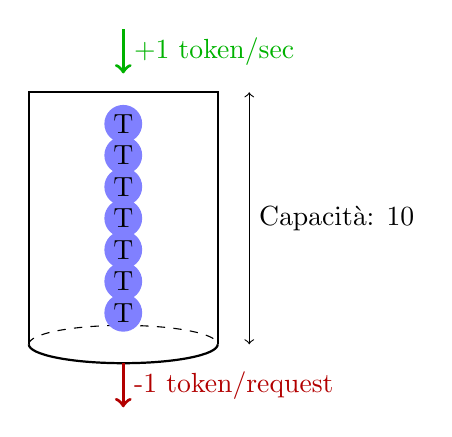
\begin{tikzpicture}[scale=0.8]
  % Bucket
  \draw[thick] (0,0) -- (0,4) -- (3,4) -- (3,0);
  \draw[thick] (0,0) arc (180:360:1.5 and 0.3);
  \draw[dashed] (0,0) arc (180:0:1.5 and 0.3);

  % Capacità
  \draw[<->] (3.5,0) -- (3.5,4) node[midway, right] {Capacità: 10};

  % Token
  \foreach \y in {0.5, 1, 1.5, 2, 2.5, 3, 3.5} {
    \fill[blue!50] (1.5, \y) circle (0.3);
    \node at (1.5, \y) {T};
  }

  % Riempimento
  \draw[->, very thick, green!70!black] (1.5, 5) -- (1.5, 4.3)
    node[midway, right] {+1 token/sec};

  % Consumo
  \draw[->, very thick, red!70!black] (1.5, -0.3) -- (1.5, -1)
    node[midway, right] {-1 token/request};
\end{tikzpicture}
\end{center}

\begin{lstlisting}[language=Python, caption=Token Bucket Implementation]
import time
import redis

class TokenBucket:
    def __init__(self, redis_client, capacity=10, refill_rate=1):
        """
        capacity: numero massimo di token
        refill_rate: token aggiunti per secondo
        """
        self.redis = redis_client
        self.capacity = capacity
        self.refill_rate = refill_rate

    def is_allowed(self, user_id):
        """Verifica se ci sono token disponibili"""
        key = f"token_bucket:{user_id}"

        # Usa script Lua per atomicità
        lua_script = """
        local key = KEYS[1]
        local capacity = tonumber(ARGV[1])
        local refill_rate = tonumber(ARGV[2])
        local now = tonumber(ARGV[3])

        local bucket = redis.call('HMGET', key, 'tokens', 'last_refill')
        local tokens = tonumber(bucket[1])
        local last_refill = tonumber(bucket[2])

        if tokens == nil then
            tokens = capacity
            last_refill = now
        end

        -- Calcola token da aggiungere
        local elapsed = now - last_refill
        local tokens_to_add = elapsed * refill_rate
        tokens = math.min(capacity, tokens + tokens_to_add)

        -- Consuma un token se disponibile
        if tokens >= 1 then
            tokens = tokens - 1
            redis.call('HMSET', key, 'tokens', tokens, 'last_refill', now)
            redis.call('EXPIRE', key, 3600)
            return 1
        else
            return 0
        end
        """

        result = self.redis.eval(
            lua_script,
            1,
            key,
            self.capacity,
            self.refill_rate,
            time.time()
        )

        return result == 1

    def get_tokens(self, user_id):
        """Ritorna token attuali"""
        key = f"token_bucket:{user_id}"
        bucket = self.redis.hmget(key, 'tokens', 'last_refill')

        if bucket[0] is None:
            return self.capacity

        tokens = float(bucket[0])
        last_refill = float(bucket[1])
        elapsed = time.time() - last_refill
        tokens = min(self.capacity, tokens + (elapsed * self.refill_rate))

        return int(tokens)
\end{lstlisting}

\subsection{Leaky Bucket}

Simile a Token Bucket ma con output a tasso costante.

\begin{lstlisting}[language=Python, caption=Leaky Bucket Implementation]
import time
import redis

class LeakyBucket:
    def __init__(self, redis_client, capacity=10, leak_rate=1):
        """
        capacity: dimensione bucket
        leak_rate: richieste processate per secondo
        """
        self.redis = redis_client
        self.capacity = capacity
        self.leak_rate = leak_rate

    def is_allowed(self, user_id):
        """Aggiungi richiesta al bucket"""
        key = f"leaky_bucket:{user_id}"

        lua_script = """
        local key = KEYS[1]
        local capacity = tonumber(ARGV[1])
        local leak_rate = tonumber(ARGV[2])
        local now = tonumber(ARGV[3])

        local bucket = redis.call('HMGET', key, 'level', 'last_leak')
        local level = tonumber(bucket[1]) or 0
        local last_leak = tonumber(bucket[2]) or now

        -- Calcola quanta acqua e' fuoriuscita
        local elapsed = now - last_leak
        local leaked = elapsed * leak_rate
        level = math.max(0, level - leaked)

        -- Prova ad aggiungere la richiesta
        if level < capacity then
            level = level + 1
            redis.call('HMSET', key, 'level', level, 'last_leak', now)
            redis.call('EXPIRE', key, 3600)
            return 1
        else
            return 0
        end
        """

        result = self.redis.eval(
            lua_script,
            1,
            key,
            self.capacity,
            self.leak_rate,
            time.time()
        )

        return result == 1
\end{lstlisting}

\subsection{Confronto Algoritmi}

\begin{table}[h]
\centering
\small
\begin{tabular}{|l|p{2.5cm}|p{2.5cm}|p{3cm}|p{2cm}|}
\hline
\textbf{Algoritmo} & \textbf{Pro} & \textbf{Contro} & \textbf{Caso d'Uso} & \textbf{Memoria} \\ \hline
Fixed Window & Semplice, efficiente & Burst al confine & API semplici & Bassa \\ \hline
Sliding Log & Preciso & Alto uso memoria & API critiche & Alta \\ \hline
Sliding Counter & Bilanciato & Approssimazione & Uso generale & Media \\ \hline
Token Bucket & Permette burst & Complesso & API con spike & Media \\ \hline
Leaky Bucket & Output uniforme & Rigido & Rate costante & Media \\ \hline
\end{tabular}
\caption{Confronto Algoritmi Rate Limiting}
\end{table}

\section{HTTP Headers per Rate Limiting}

\subsection{Standard Headers}

\begin{lstlisting}[caption=Headers di Rate Limiting (Draft IETF)]
RateLimit-Limit: 100
RateLimit-Remaining: 85
RateLimit-Reset: 1699876543
\end{lstlisting}

\subsection{Headers Legacy (X- prefix)}

Molte API usano ancora headers con prefisso \texttt{X-}:

\begin{lstlisting}[caption=Headers X-RateLimit-*]
X-RateLimit-Limit: 100
X-RateLimit-Remaining: 85
X-RateLimit-Reset: 1699876543
\end{lstlisting}

\subsection{Descrizione Headers}

\begin{table}[h]
\centering
\begin{tabular}{|l|p{10cm}|}
\hline
\textbf{Header} & \textbf{Descrizione} \\ \hline
\texttt{RateLimit-Limit} & Numero massimo di richieste consentite nella finestra \\ \hline
\texttt{RateLimit-Remaining} & Numero di richieste rimanenti nella finestra corrente \\ \hline
\texttt{RateLimit-Reset} & Unix timestamp di quando il limite si resetterà \\ \hline
\texttt{Retry-After} & Secondi da attendere prima di riprovare (usato con 429) \\ \hline
\end{tabular}
\caption{HTTP Headers Rate Limiting}
\end{table}

\subsection{Response di Successo}

\begin{lstlisting}[caption=Response 200 con Rate Limit Headers]
HTTP/1.1 200 OK
Content-Type: application/json
RateLimit-Limit: 100
RateLimit-Remaining: 85
RateLimit-Reset: 1699876543

{
  "data": {
    "users": [...]
  }
}
\end{lstlisting}

\subsection{Response quando Limite Superato}

\begin{lstlisting}[caption=Response 429 Too Many Requests]
HTTP/1.1 429 Too Many Requests
Content-Type: application/json
RateLimit-Limit: 100
RateLimit-Remaining: 0
RateLimit-Reset: 1699876543
Retry-After: 43

{
  "error": {
    "code": "rate_limit_exceeded",
    "message": "API rate limit exceeded",
    "limit": 100,
    "remaining": 0,
    "reset_at": "2023-11-13T12:35:43Z",
    "retry_after": 43
  }
}
\end{lstlisting}

\section{Implementazione Middleware}

\subsection{Express.js Middleware}

\begin{lstlisting}[language=JavaScript, caption=Rate Limiting Middleware Node.js]
const redis = require('redis');
const client = redis.createClient();

const rateLimitMiddleware = (options = {}) => {
  const {
    windowMs = 60000,      // 1 minuto
    max = 100,             // 100 richieste
    keyGenerator = (req) => req.ip,
    handler = (req, res) => {
      res.status(429).json({
        error: 'Too many requests, please try again later.'
      });
    }
  } = options;

  return async (req, res, next) => {
    const key = `rate_limit:${keyGenerator(req)}`;
    const now = Date.now();
    const windowStart = now - windowMs;

    try {
      // Rimuovi entry vecchie
      await client.zRemRangeByScore(key, 0, windowStart);

      // Conta richieste nella finestra
      const count = await client.zCard(key);

      // Headers
      res.setHeader('RateLimit-Limit', max);
      res.setHeader('RateLimit-Remaining', Math.max(0, max - count - 1));
      res.setHeader('RateLimit-Reset',
        Math.ceil((now + windowMs) / 1000));

      if (count >= max) {
        res.setHeader('Retry-After', Math.ceil(windowMs / 1000));
        return handler(req, res);
      }

      // Aggiungi richiesta corrente
      await client.zAdd(key, { score: now, value: `${now}` });
      await client.expire(key, Math.ceil(windowMs / 1000));

      next();
    } catch (error) {
      console.error('Rate limit error:', error);
      next(); // Fail open in caso di errore
    }
  };
};

// Utilizzo
const express = require('express');
const app = express();

// Rate limit globale
app.use(rateLimitMiddleware({
  windowMs: 60000,
  max: 100
}));

// Rate limit specifico per login
app.post('/api/login',
  rateLimitMiddleware({
    windowMs: 300000,  // 5 minuti
    max: 5,            // 5 tentativi
    keyGenerator: (req) => req.body.email || req.ip
  }),
  (req, res) => {
    // Login logic
  }
);
\end{lstlisting}

\subsection{Flask Decorator}

\begin{lstlisting}[language=Python, caption=Rate Limiting Decorator Python/Flask]
from functools import wraps
from flask import request, jsonify
import redis
import time

redis_client = redis.Redis(host='localhost', port=6379, db=0)

def rate_limit(max_requests=100, window_seconds=60,
               key_func=lambda: request.remote_addr):
    """
    Decorator per rate limiting
    """
    def decorator(f):
        @wraps(f)
        def wrapped(*args, **kwargs):
            # Genera chiave
            key = f"rate_limit:{key_func()}"
            now = time.time()
            window_start = now - window_seconds

            # Rimuovi richieste fuori finestra
            redis_client.zremrangebyscore(key, 0, window_start)

            # Conta richieste
            current_count = redis_client.zcard(key)

            # Calcola reset time
            reset_time = int(now + window_seconds)

            # Headers
            from flask import make_response
            response = None

            if current_count >= max_requests:
                # Limite superato
                response = make_response(jsonify({
                    'error': 'rate_limit_exceeded',
                    'message': 'Too many requests',
                    'limit': max_requests,
                    'retry_after': window_seconds
                }), 429)
                response.headers['Retry-After'] = str(window_seconds)
            else:
                # Aggiungi richiesta
                redis_client.zadd(key, {str(now): now})
                redis_client.expire(key, window_seconds)

                # Esegui funzione
                response = make_response(f(*args, **kwargs))

            # Aggiungi headers rate limit
            response.headers['RateLimit-Limit'] = str(max_requests)
            response.headers['RateLimit-Remaining'] = str(
                max(0, max_requests - current_count - 1)
            )
            response.headers['RateLimit-Reset'] = str(reset_time)

            return response

        return wrapped
    return decorator

# Utilizzo
@app.route('/api/data')
@rate_limit(max_requests=100, window_seconds=60)
def get_data():
    return jsonify({'data': 'some data'})

@app.route('/api/login', methods=['POST'])
@rate_limit(
    max_requests=5,
    window_seconds=300,
    key_func=lambda: request.json.get('email', request.remote_addr)
)
def login():
    # Login logic
    return jsonify({'token': 'abc123'})
\end{lstlisting}

\section{Rate Limiting Avanzato}

\subsection{Limiti per Piano di Servizio}

\begin{lstlisting}[language=Python, caption=Rate Limit basato su Piano Utente]
RATE_LIMIT_TIERS = {
    'free': {
        'requests_per_hour': 100,
        'requests_per_day': 1000,
        'burst': 10
    },
    'pro': {
        'requests_per_hour': 1000,
        'requests_per_day': 20000,
        'burst': 50
    },
    'enterprise': {
        'requests_per_hour': 10000,
        'requests_per_day': 500000,
        'burst': 200
    }
}

def get_user_tier(user_id):
    """Ottieni tier dell'utente dal database"""
    # Query database
    user = db.users.find_one({'id': user_id})
    return user.get('tier', 'free')

def check_rate_limit(user_id):
    """Verifica rate limit con tier-based limits"""
    tier = get_user_tier(user_id)
    limits = RATE_LIMIT_TIERS[tier]

    # Verifica limite orario
    hourly_key = f"rate:{user_id}:hour:{int(time.time() / 3600)}"
    hourly_count = redis_client.incr(hourly_key)
    redis_client.expire(hourly_key, 3600)

    if hourly_count > limits['requests_per_hour']:
        return False, 'hourly_limit_exceeded'

    # Verifica limite giornaliero
    daily_key = f"rate:{user_id}:day:{int(time.time() / 86400)}"
    daily_count = redis_client.incr(daily_key)
    redis_client.expire(daily_key, 86400)

    if daily_count > limits['requests_per_day']:
        return False, 'daily_limit_exceeded'

    return True, None
\end{lstlisting}

\subsection{Limiti per Endpoint}

\begin{lstlisting}[language=Python, caption=Rate Limit Differenziato per Endpoint]
ENDPOINT_LIMITS = {
    '/api/search': {
        'max_requests': 20,
        'window_seconds': 60
    },
    '/api/upload': {
        'max_requests': 5,
        'window_seconds': 60
    },
    '/api/users': {
        'max_requests': 100,
        'window_seconds': 60
    },
    'default': {
        'max_requests': 60,
        'window_seconds': 60
    }
}

def get_endpoint_limit(endpoint):
    """Ottieni configurazione rate limit per endpoint"""
    return ENDPOINT_LIMITS.get(endpoint, ENDPOINT_LIMITS['default'])

@app.before_request
def check_endpoint_rate_limit():
    """Middleware per rate limiting per endpoint"""
    endpoint = request.endpoint
    user_id = get_current_user_id()

    config = get_endpoint_limit(endpoint)
    key = f"rate:{user_id}:{endpoint}"

    if not is_allowed(key, config['max_requests'],
                      config['window_seconds']):
        return jsonify({
            'error': 'rate_limit_exceeded',
            'endpoint': endpoint,
            'limit': config['max_requests']
        }), 429
\end{lstlisting}

\subsection{Limiti Dinamici}

\begin{lstlisting}[language=Python, caption=Rate Limiting Dinamico Basato su Carico]
def get_dynamic_rate_limit():
    """Calcola rate limit dinamico basato sul carico server"""

    # Ottieni metriche sistema
    cpu_usage = psutil.cpu_percent()
    memory_usage = psutil.virtual_memory().percent

    # Calcola limite basato su carico
    if cpu_usage > 80 or memory_usage > 80:
        # Carico alto: riduci limite
        return 50
    elif cpu_usage > 60 or memory_usage > 60:
        # Carico medio
        return 100
    else:
        # Carico basso: limite normale
        return 200

def adaptive_rate_limit(user_id):
    """Rate limiting adattivo"""
    limit = get_dynamic_rate_limit()
    key = f"rate:adaptive:{user_id}"

    return is_allowed(key, limit, window_seconds=60)
\end{lstlisting}

\section{Best Practices}

\subsection{Comunicazione Chiara}

\begin{tcolorbox}[title=Documentare i Limiti]
\begin{itemize}
\item Documentare chiaramente i rate limits nella API docs
\item Includere limiti per ogni piano di servizio
\item Specificare come vengono contate le richieste
\item Fornire esempi di headers di risposta
\end{itemize}
\end{tcolorbox}

\subsection{Graceful Degradation}

\begin{lstlisting}[caption=Response con Suggerimenti]
{
  "error": {
    "code": "rate_limit_exceeded",
    "message": "You have exceeded your rate limit",
    "current_usage": 1050,
    "limit": 1000,
    "reset_at": "2023-11-13T13:00:00Z",
    "suggestions": [
      "Wait 15 minutes before retrying",
      "Upgrade to Pro plan for higher limits",
      "Use webhooks instead of polling"
    ],
    "documentation_url": "https://docs.example.com/rate-limits"
  }
}
\end{lstlisting}

\subsection{Monitoring}

\begin{lstlisting}[language=Python, caption=Logging e Metriche Rate Limiting]
import logging
from prometheus_client import Counter, Histogram

# Metriche Prometheus
rate_limit_exceeded = Counter(
    'rate_limit_exceeded_total',
    'Total rate limit exceeded events',
    ['user_tier', 'endpoint']
)

rate_limit_usage = Histogram(
    'rate_limit_usage_percentage',
    'Rate limit usage percentage',
    ['user_tier']
)

def log_rate_limit_event(user_id, tier, endpoint, exceeded):
    """Log eventi rate limiting"""

    if exceeded:
        logging.warning(
            f"Rate limit exceeded - User: {user_id}, "
            f"Tier: {tier}, Endpoint: {endpoint}"
        )
        rate_limit_exceeded.labels(
            user_tier=tier,
            endpoint=endpoint
        ).inc()

    # Log usage
    usage = get_current_usage(user_id)
    limit = get_limit(tier)
    percentage = (usage / limit) * 100

    rate_limit_usage.labels(user_tier=tier).observe(percentage)
\end{lstlisting>

\section{OpenAPI Specification}

\begin{lstlisting}[caption=Documentare Rate Limiting in OpenAPI]
openapi: 3.0.0
info:
  title: Rate Limited API
  version: 1.0.0
  description: |
    ## Rate Limiting

    This API implements rate limiting to ensure fair usage.

    ### Limits by Plan

    | Plan       | Requests/Hour | Requests/Day |
    |------------|---------------|--------------|
    | Free       | 100           | 1,000        |
    | Pro        | 1,000         | 20,000       |
    | Enterprise | 10,000        | 500,000      |

    ### Headers

    All responses include rate limit headers:
    - `RateLimit-Limit`: Maximum requests allowed
    - `RateLimit-Remaining`: Requests remaining
    - `RateLimit-Reset`: Unix timestamp of reset

    ### 429 Response

    When limit is exceeded, API returns 429 status with Retry-After header.

paths:
  /api/search:
    get:
      summary: Search resources
      description: |
        Search endpoint with stricter rate limiting (20 req/min)
      responses:
        '200':
          description: Search results
          headers:
            RateLimit-Limit:
              schema:
                type: integer
              description: Maximum requests per window
            RateLimit-Remaining:
              schema:
                type: integer
              description: Remaining requests in window
            RateLimit-Reset:
              schema:
                type: integer
              description: Unix timestamp when limit resets
          content:
            application/json:
              schema:
                type: object

        '429':
          description: Rate limit exceeded
          headers:
            RateLimit-Limit:
              schema:
                type: integer
            RateLimit-Remaining:
              schema:
                type: integer
              example: 0
            RateLimit-Reset:
              schema:
                type: integer
            Retry-After:
              schema:
                type: integer
              description: Seconds to wait before retrying
          content:
            application/json:
              schema:
                type: object
                properties:
                  error:
                    type: object
                    properties:
                      code:
                        type: string
                        example: rate_limit_exceeded
                      message:
                        type: string
                      limit:
                        type: integer
                      reset_at:
                        type: string
                        format: date-time
\end{lstlisting}

\section{Testing}

\subsection{Script di Test}

\begin{lstlisting}[language=bash, caption=Test Rate Limiting con cURL]
#!/bin/bash

API_URL="https://api.example.com/data"
TOKEN="your-api-token"

echo "=== Rate Limit Test ==="

# Invia richieste fino al limite
for i in {1..105}; do
  echo "Request #$i"

  response=$(curl -s -w "\n%{http_code}" \
    -H "Authorization: Bearer $TOKEN" \
    "$API_URL")

  status_code=$(echo "$response" | tail -n1)
  body=$(echo "$response" | head -n-1)

  # Estrai headers (richiede -i flag in curl)
  limit=$(echo "$body" | jq -r '.headers."RateLimit-Limit" // empty')
  remaining=$(echo "$body" | jq -r '.headers."RateLimit-Remaining" // empty')

  echo "  Status: $status_code"
  echo "  Remaining: $remaining"

  if [ "$status_code" == "429" ]; then
    echo "  RATE LIMIT HIT!"
    retry_after=$(echo "$body" | jq -r '.error.retry_after')
    echo "  Retry after: $retry_after seconds"
    break
  fi

  # Pausa breve
  sleep 0.1
done
\end{lstlisting}

\subsection{Test Unitari}

\begin{lstlisting}[language=Python, caption=Unit Test Rate Limiter]
import unittest
import time
from rate_limiter import FixedWindowRateLimiter

class TestRateLimiter(unittest.TestCase):
    def setUp(self):
        self.redis = fakeredis.FakeStrictRedis()
        self.limiter = FixedWindowRateLimiter(
            self.redis,
            window_seconds=60,
            max_requests=10
        )

    def test_allows_requests_under_limit(self):
        """Verifica che richieste sotto il limite siano consentite"""
        user_id = "test_user"

        for i in range(10):
            self.assertTrue(self.limiter.is_allowed(user_id))

    def test_blocks_requests_over_limit(self):
        """Verifica che richieste oltre il limite siano bloccate"""
        user_id = "test_user"

        # Riempi il limite
        for i in range(10):
            self.limiter.is_allowed(user_id)

        # La 11esima deve essere bloccata
        self.assertFalse(self.limiter.is_allowed(user_id))

    def test_resets_after_window(self):
        """Verifica reset dopo la finestra"""
        user_id = "test_user"

        # Riempi limite
        for i in range(10):
            self.limiter.is_allowed(user_id)

        # Simula passaggio tempo
        time.sleep(61)

        # Deve permettere di nuovo
        self.assertTrue(self.limiter.is_allowed(user_id))

if __name__ == '__main__':
    unittest.main()
\end{lstlisting}

\section{Riepilogo}

\begin{tcolorbox}[title=Checklist Rate Limiting]
\begin{itemize}
\item[$\square$] Scegli algoritmo appropriato per il tuo caso d'uso
\item[$\square$] Implementa rate limiting a più livelli (IP, user, endpoint)
\item[$\square$] Usa headers standard (RateLimit-*)
\item[$\square$] Fornisci response 429 chiare con Retry-After
\item[$\square$] Documenta limiti chiaramente
\item[$\square$] Monitora e logga eventi di rate limiting
\item[$\square$] Implementa limiti differenziati per piani
\item[$\square$] Testa il comportamento sotto carico
\item[$\square$] Considera fail-open per garantire disponibilità
\item[$\square$] Fornisci meccanismi di upgrade/whitelist
\end{itemize}
\end{tcolorbox}
